\subsection{High Energy Sidebands}
\label{sec:HighEnergySidebands}

The first set of sub-sidebands to inspect is obtained by selecting the high energy regions of the two far sidebands. These are defined in the case of the 1eNp selection as events with a reconstructed energy greater than 1.05~GeV and in the case of the 1e0p, events with reconstructed energies above 0.90~GeV.

The three main variables of interest in the case of the 1eNp selection are the reconstructed neutrino energy, shown with run 1-3 data in Figure~\ref{fig:HighEnergy1eNp_reco_e}, and the two BDT scores, shown in Figures~\ref{fig:HighEnergy1eNp_pi0_score}, and ~\ref{fig:HighEnergy1eNp_nonpi0_score}.

\begin{figure}[H]
    \centering
    \begin{subfigure}{0.33\linewidth}
    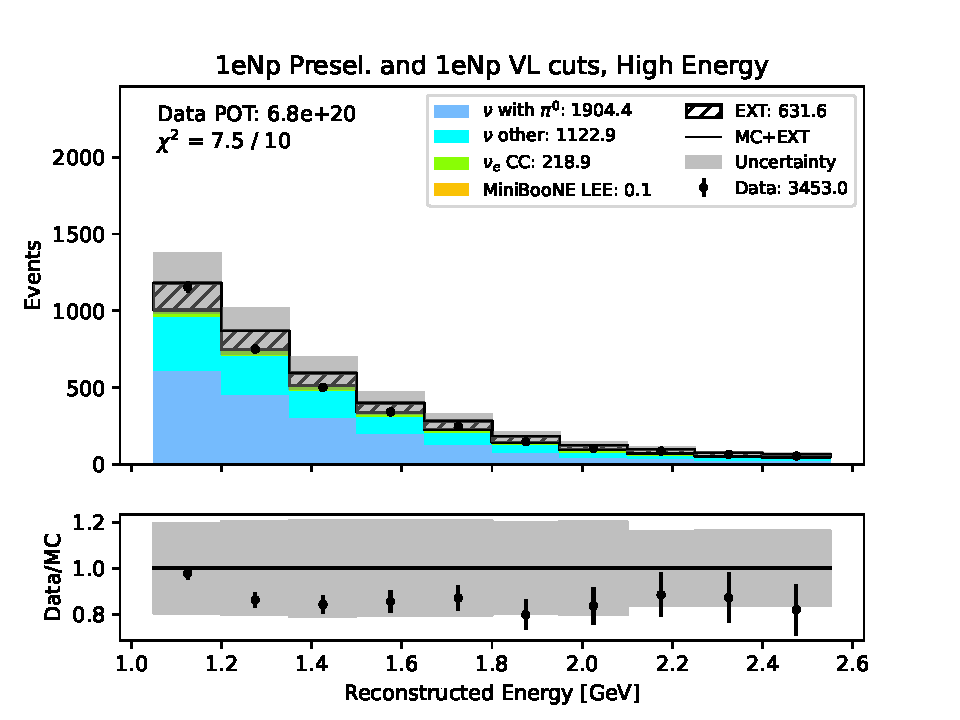
\includegraphics[width=\linewidth]{technote/Sidebands/Figures/FarSideband/far_sideband_reco_e_run123_NP_NP_HIGH_ENERGY.pdf}
    \caption{$\nu_e$ preselection, runs 1-3.}
    \end{subfigure}%
    \begin{subfigure}{0.33\linewidth}
    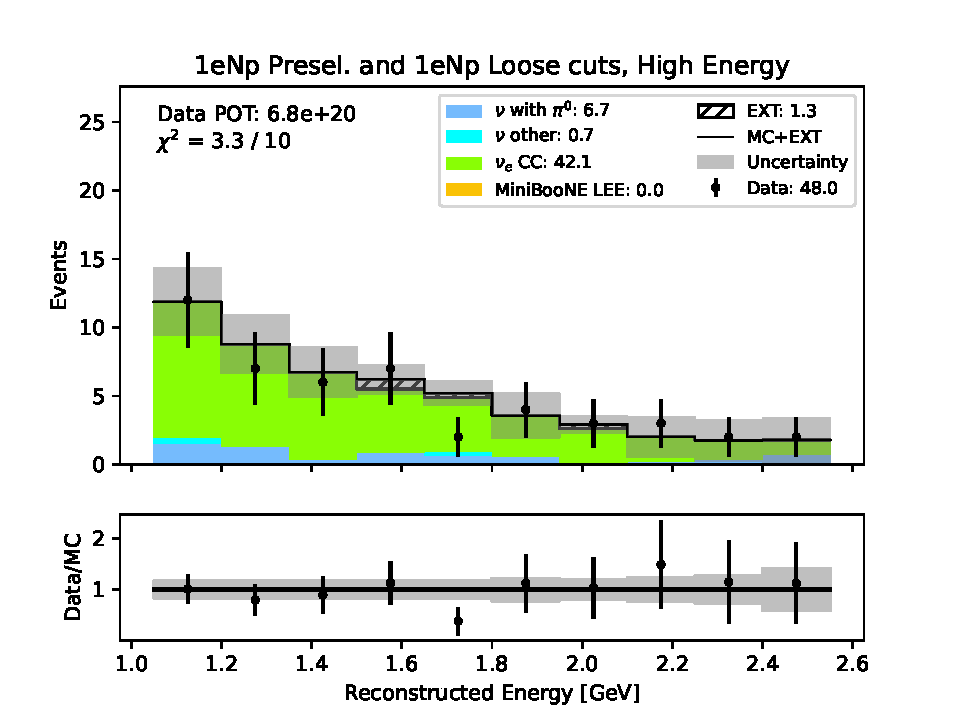
\includegraphics[width=\linewidth]{technote/Sidebands/Figures/FarSideband/far_sideband_reco_e_run123_NP_NPL_HIGH_ENERGY.pdf}
    \caption{1eNp loose selection, runs 1-3.}
    \end{subfigure}%
    \begin{subfigure}{0.33\linewidth}
    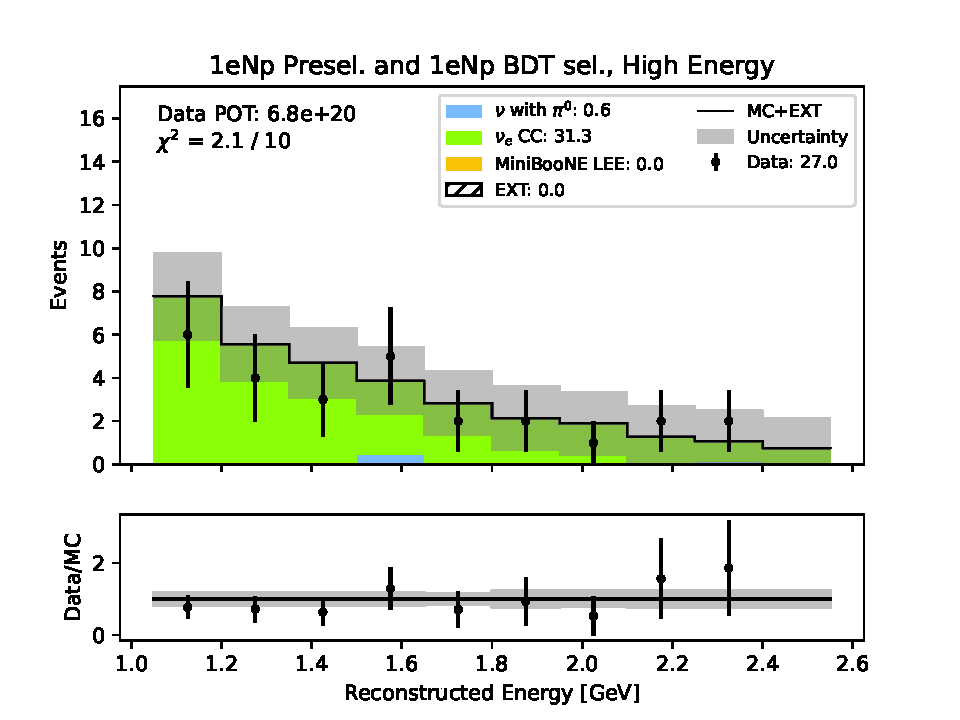
\includegraphics[width=\linewidth]{technote/Sidebands/Figures/FarSideband/far_sideband_reco_e_run123_NP_NPBDT_HIGH_ENERGY.pdf}
    \caption{1eNp BDT selection, runs 1-3.}
    \end{subfigure}
    \begin{subfigure}{0.33\linewidth}
    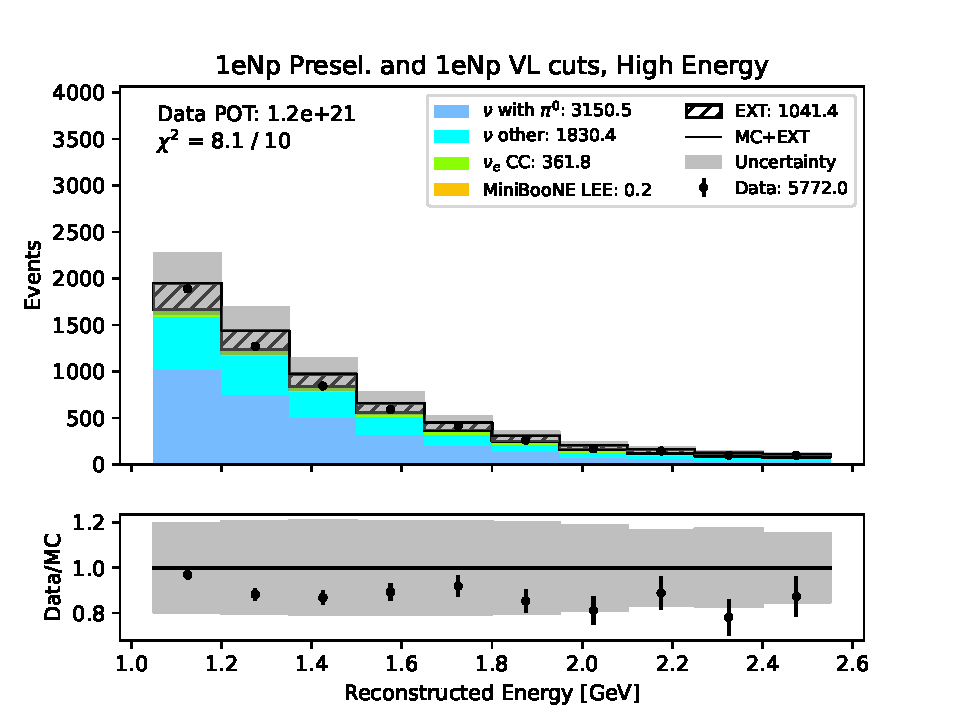
\includegraphics[width=\linewidth]{technote/Sidebands/Figures/FarSideband/far_sideband_reco_e_run1234a4b4c4d5_NP_NP_HIGH_ENERGY.pdf}
    \caption{$\nu_e$ preselection, runs 1-5.}
    \end{subfigure}%
    \begin{subfigure}{0.33\linewidth}
    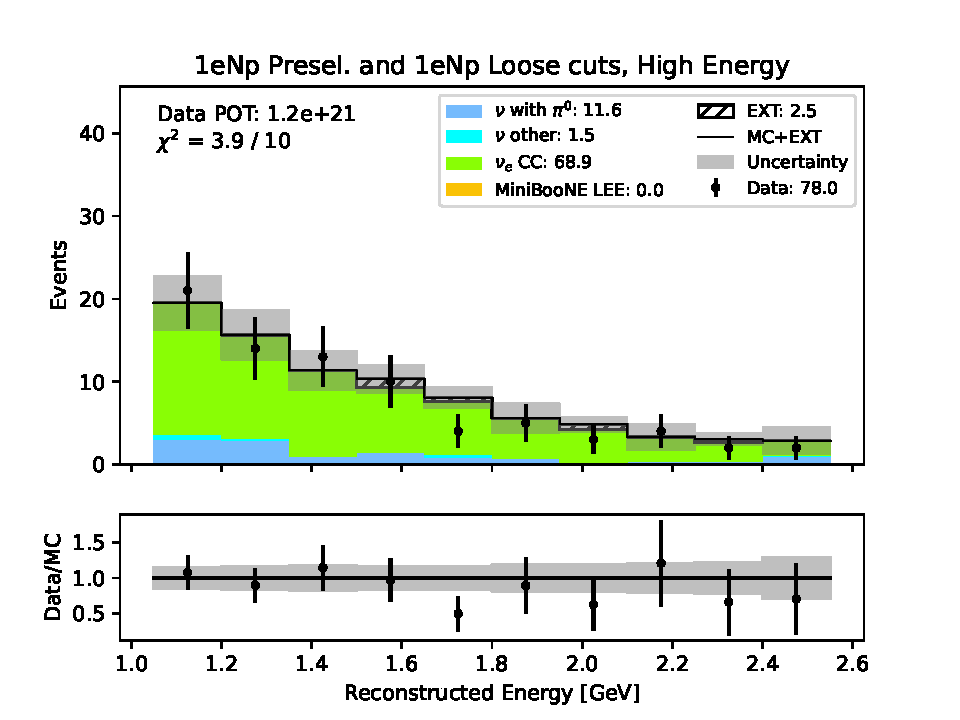
\includegraphics[width=\linewidth]{technote/Sidebands/Figures/FarSideband/far_sideband_reco_e_run1234a4b4c4d5_NP_NPL_HIGH_ENERGY.pdf}
    \caption{1eNp loose selection, runs 1-5.}
    \end{subfigure}%
    \begin{subfigure}{0.33\linewidth}
    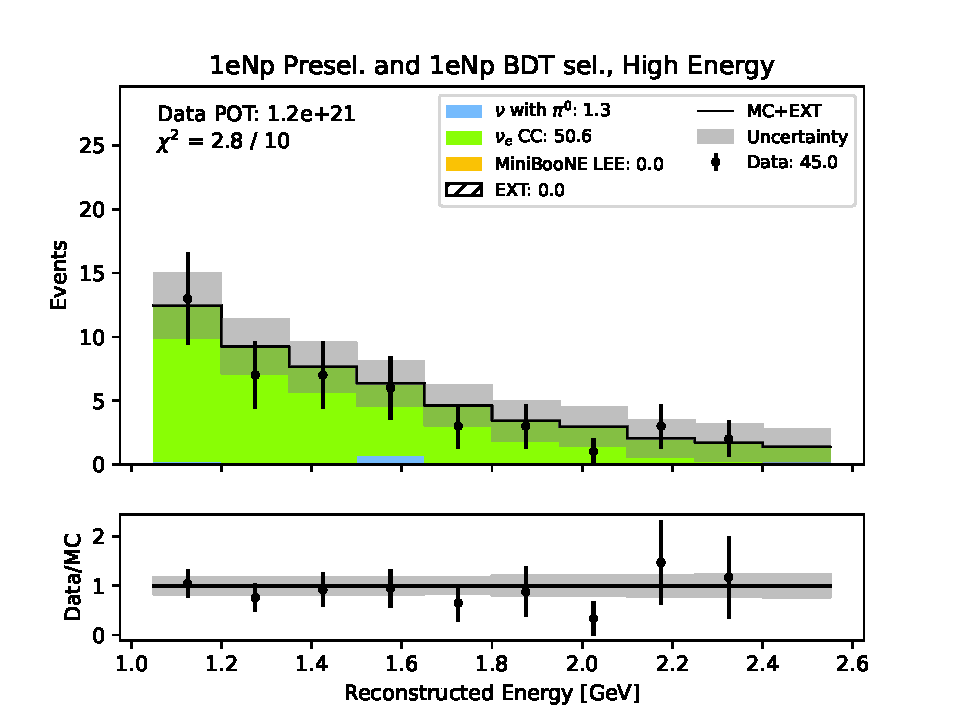
\includegraphics[width=\linewidth]{technote/Sidebands/Figures/FarSideband/far_sideband_reco_e_run1234a4b4c4d5_NP_NPBDT_HIGH_ENERGY.pdf}
    \caption{1eNp BDT selection, runs 1-5.}
    \end{subfigure}
    \caption{Reconstructed neutrino energy in the 1eNp high energy sideband.}
     \label{fig:HighEnergy1eNp_reco_e}
\end{figure}

\begin{figure}[H]
    \centering
    \begin{subfigure}{0.33\linewidth}
    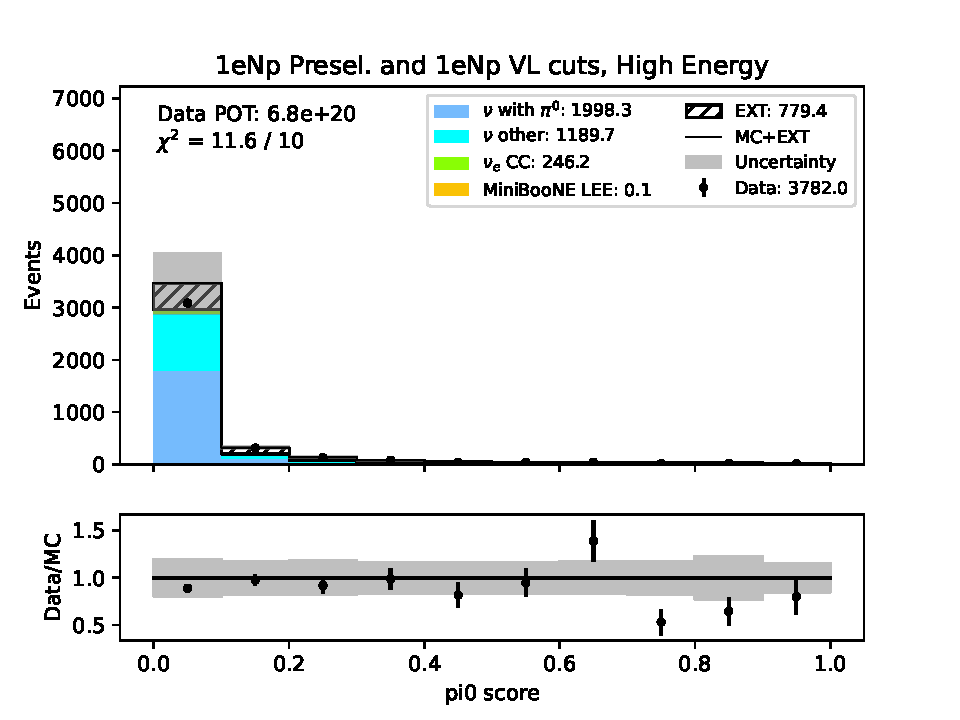
\includegraphics[width=\linewidth]{technote/Sidebands/Figures/FarSideband/far_sideband_pi0_score_run123_NP_NP_HIGH_ENERGY.pdf}
    \caption{$\nu_e$ preselection, runs 1-3.}
    \end{subfigure}%
    \begin{subfigure}{0.33\linewidth}
    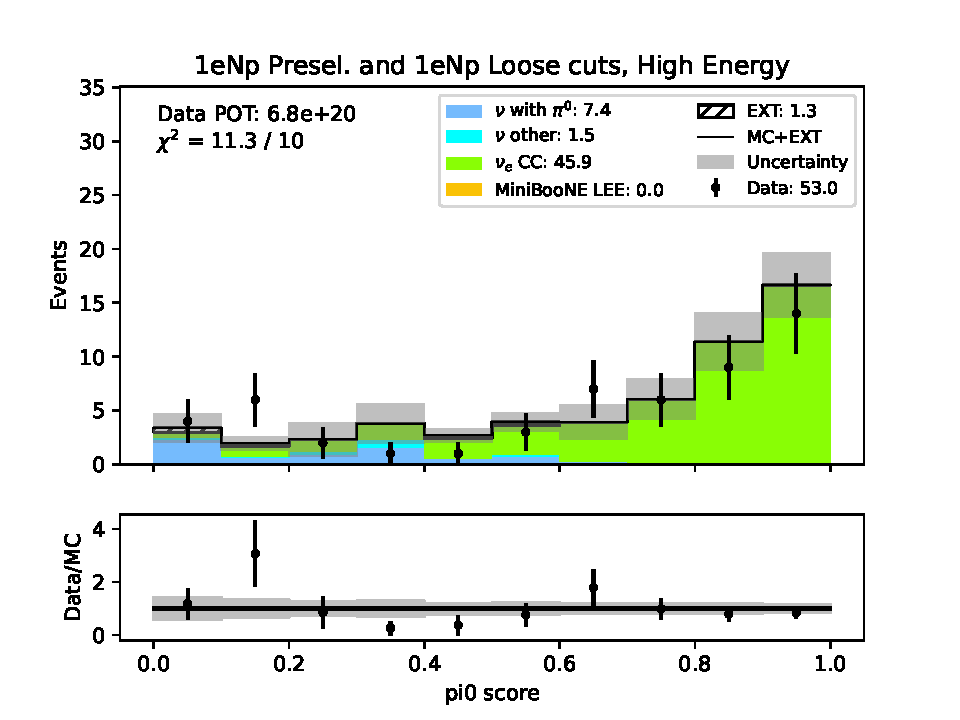
\includegraphics[width=\linewidth]{technote/Sidebands/Figures/FarSideband/far_sideband_pi0_score_run123_NP_NPL_HIGH_ENERGY.pdf}
    \caption{1eNp loose selection, runs 1-3.}
    \end{subfigure}%
    \begin{subfigure}{0.33\linewidth}
    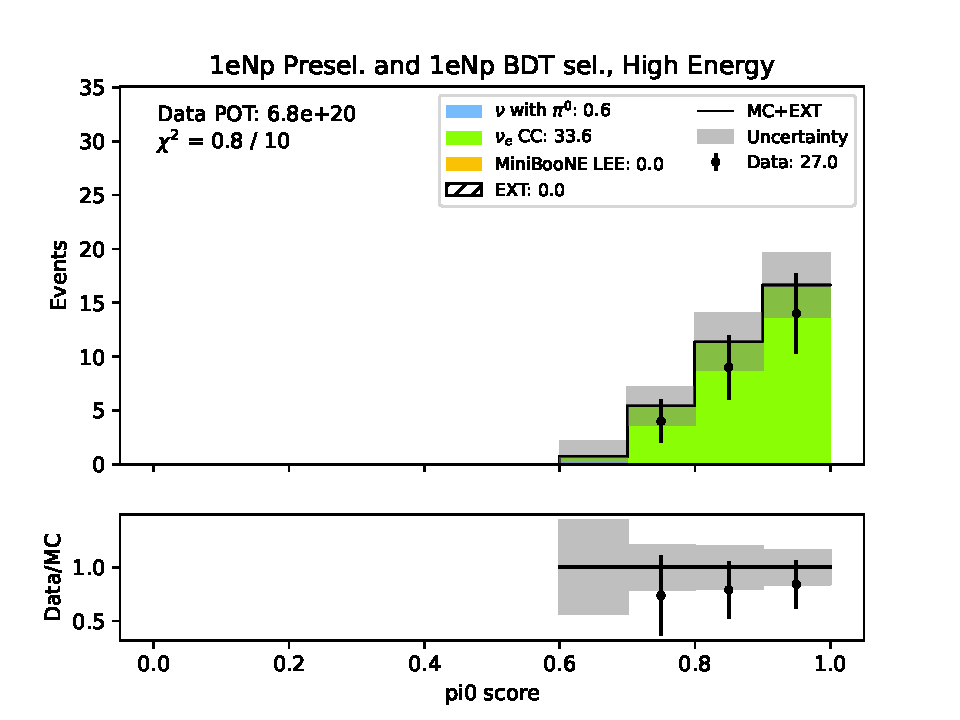
\includegraphics[width=\linewidth]{technote/Sidebands/Figures/FarSideband/far_sideband_pi0_score_run123_NP_NPBDT_HIGH_ENERGY.pdf}
    \caption{1eNp BDT selection, runs 1-3.}
    \end{subfigure}
    \begin{subfigure}{0.33\linewidth}
    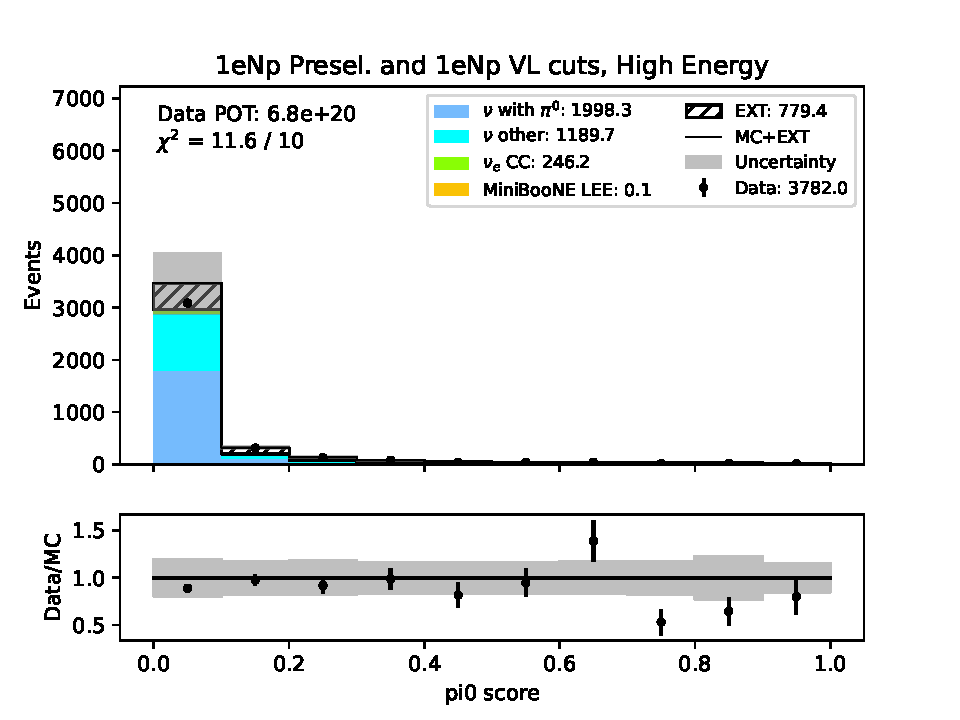
\includegraphics[width=\linewidth]{technote/Sidebands/Figures/FarSideband/far_sideband_pi0_score_run123_NP_NP_HIGH_ENERGY.pdf}
    \caption{$\nu_e$ preselection, runs 1-5.}
    \end{subfigure}%
    \begin{subfigure}{0.33\linewidth}
    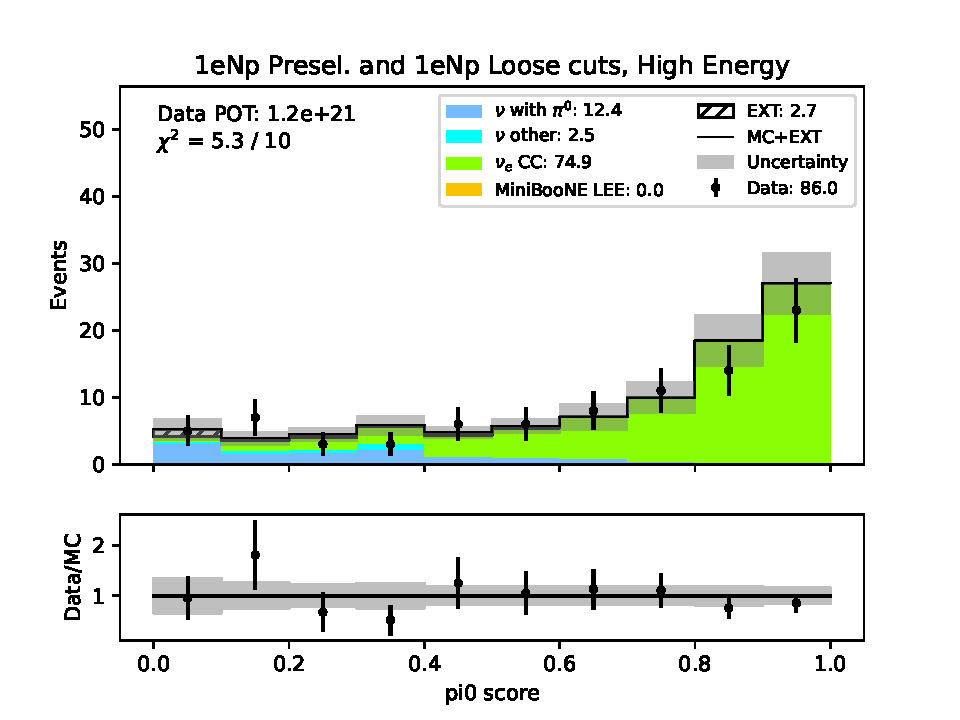
\includegraphics[width=\linewidth]{technote/Sidebands/Figures/FarSideband/far_sideband_pi0_score_run1234a4b4c4d5_NP_NPL_HIGH_ENERGY.pdf}
    \caption{1eNp loose selection, runs 1-5.}
    \end{subfigure}%
    \begin{subfigure}{0.33\linewidth}
    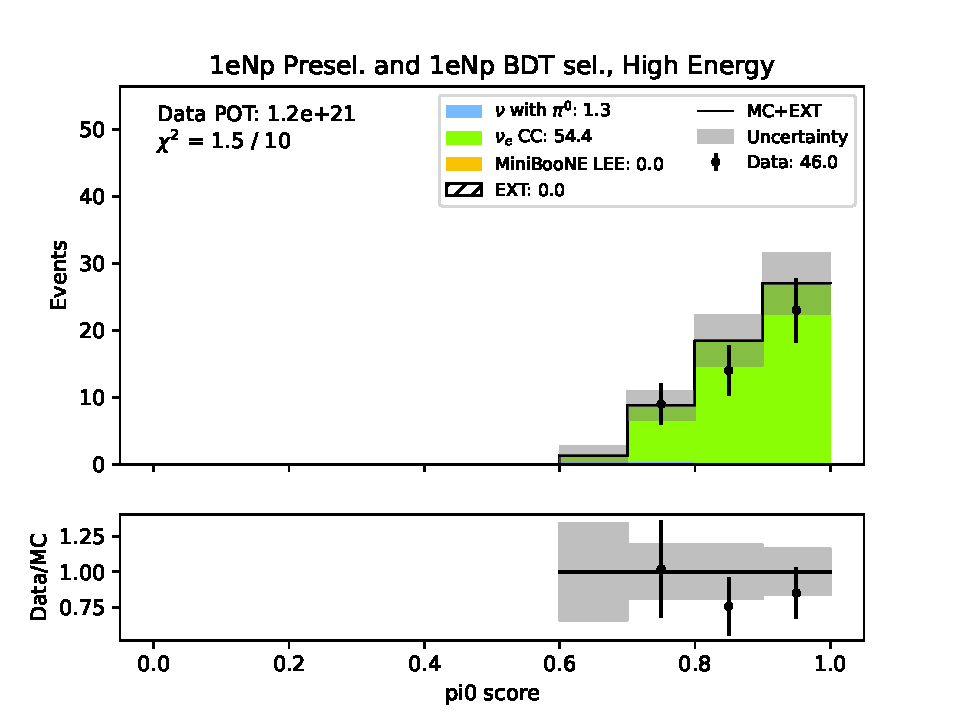
\includegraphics[width=\linewidth]{technote/Sidebands/Figures/FarSideband/far_sideband_pi0_score_run1234a4b4c4d5_NP_NPBDT_HIGH_ENERGY.pdf}
    \caption{1eNp BDT selection, runs 1-5.}
    \end{subfigure}
    \caption{Reconstructed neutrino energy in the 1eNp high energy sideband.}
    \label{fig:HighEnergy1eNp_pi0_score}
\end{figure}

\begin{figure}[H]
    \centering
    \begin{subfigure}{0.33\linewidth}
    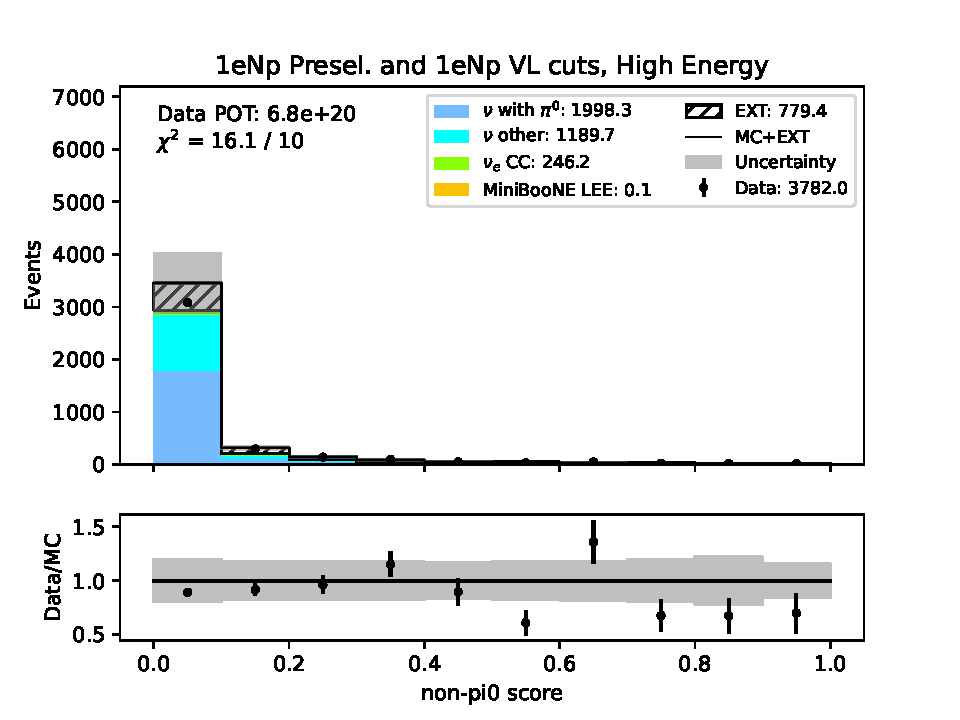
\includegraphics[width=\linewidth]{technote/Sidebands/Figures/FarSideband/far_sideband_nonpi0_score_run123_NP_NP_HIGH_ENERGY.pdf}
    \caption{$\nu_e$ preselection, runs 1-3.}
    \end{subfigure}%
    \begin{subfigure}{0.33\linewidth}
    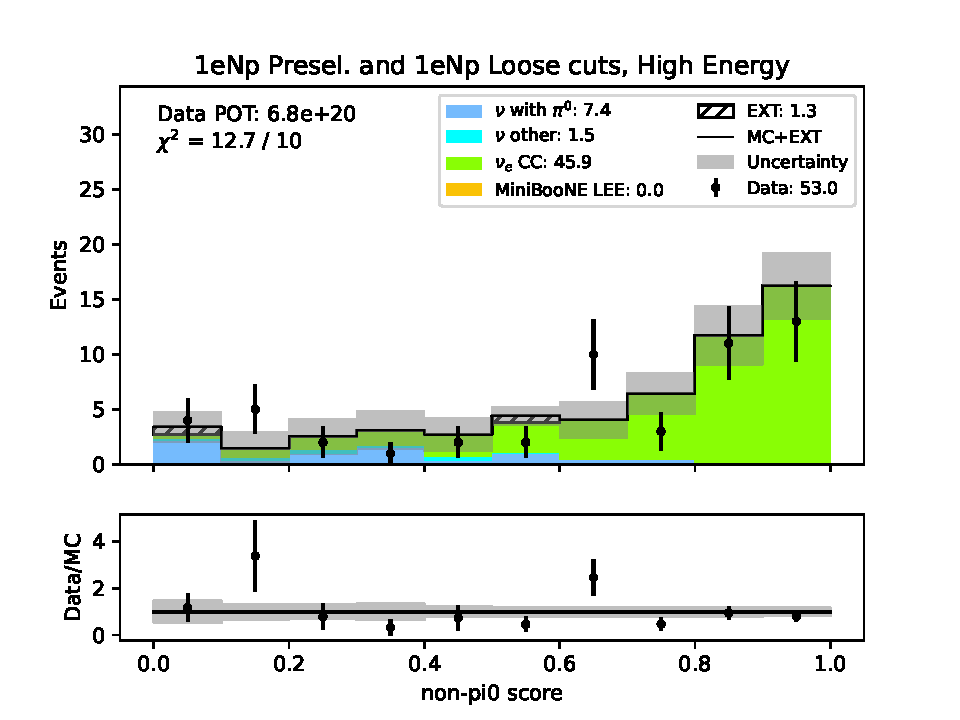
\includegraphics[width=\linewidth]{technote/Sidebands/Figures/FarSideband/far_sideband_nonpi0_score_run123_NP_NPL_HIGH_ENERGY.pdf}
    \caption{1eNp loose selection, runs 1-3.}
    \end{subfigure}%
    \begin{subfigure}{0.33\linewidth}
    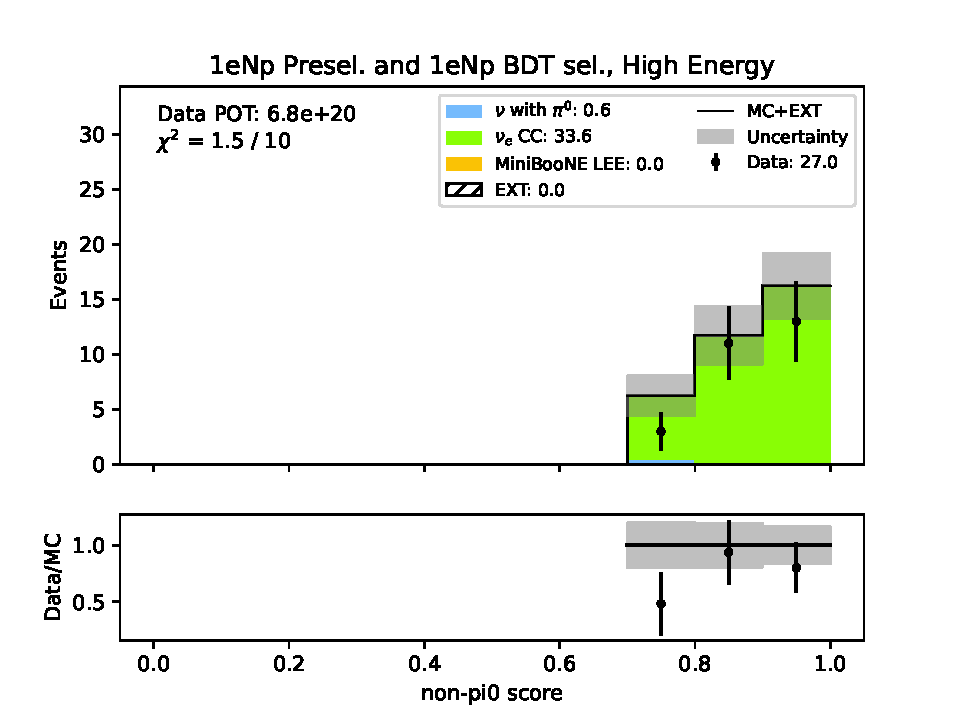
\includegraphics[width=\linewidth]{technote/Sidebands/Figures/FarSideband/far_sideband_nonpi0_score_run123_NP_NPBDT_HIGH_ENERGY.pdf}
    \caption{1eNp BDT selection, runs 1-3.}
    \end{subfigure}
    \begin{subfigure}{0.33\linewidth}
    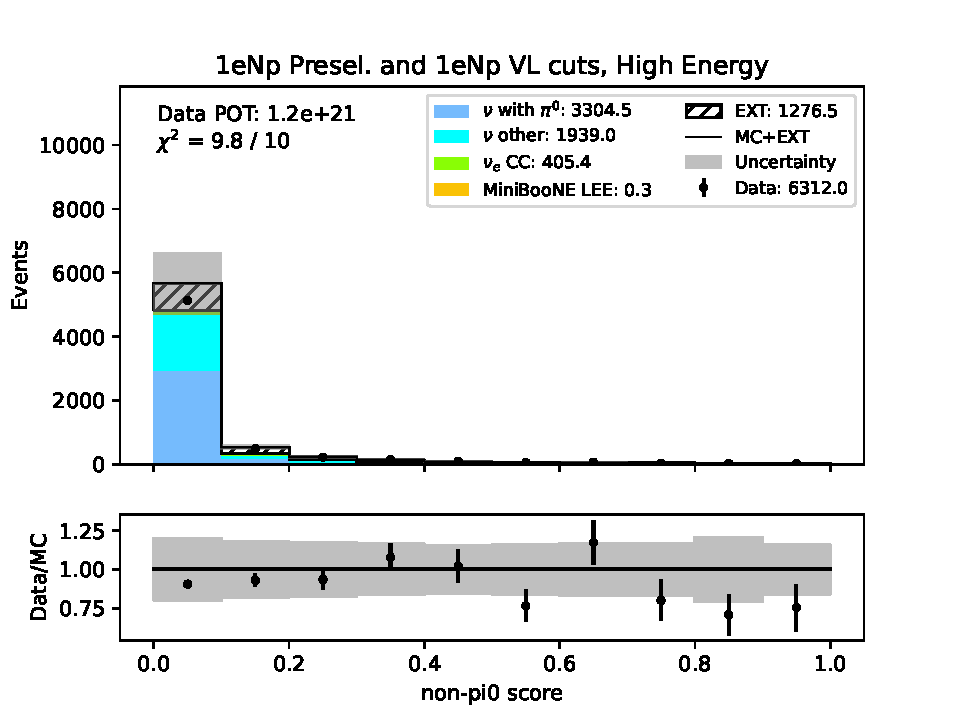
\includegraphics[width=\linewidth]{technote/Sidebands/Figures/FarSideband/far_sideband_nonpi0_score_run1234a4b4c4d5_NP_NP_HIGH_ENERGY.pdf}
    \caption{$\nu_e$ preselection, runs 1-5.}
    \end{subfigure}%
    \begin{subfigure}{0.33\linewidth}
    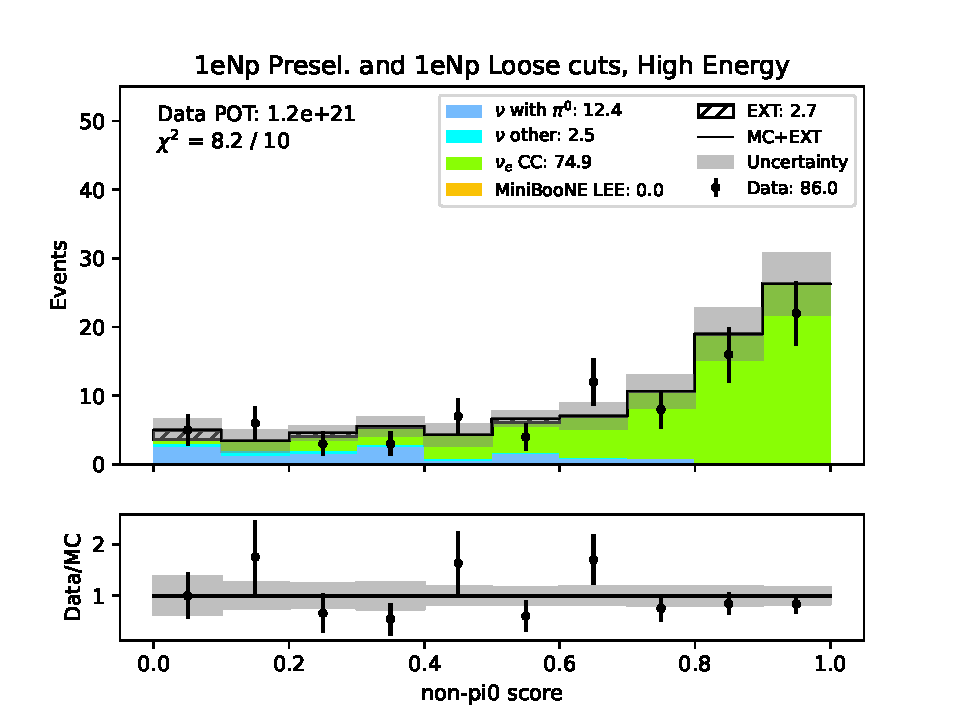
\includegraphics[width=\linewidth]{technote/Sidebands/Figures/FarSideband/far_sideband_nonpi0_score_run1234a4b4c4d5_NP_NPL_HIGH_ENERGY.pdf}
    \caption{1eNp loose selection, runs 1-5.}
    \end{subfigure}%
    \begin{subfigure}{0.33\linewidth}
    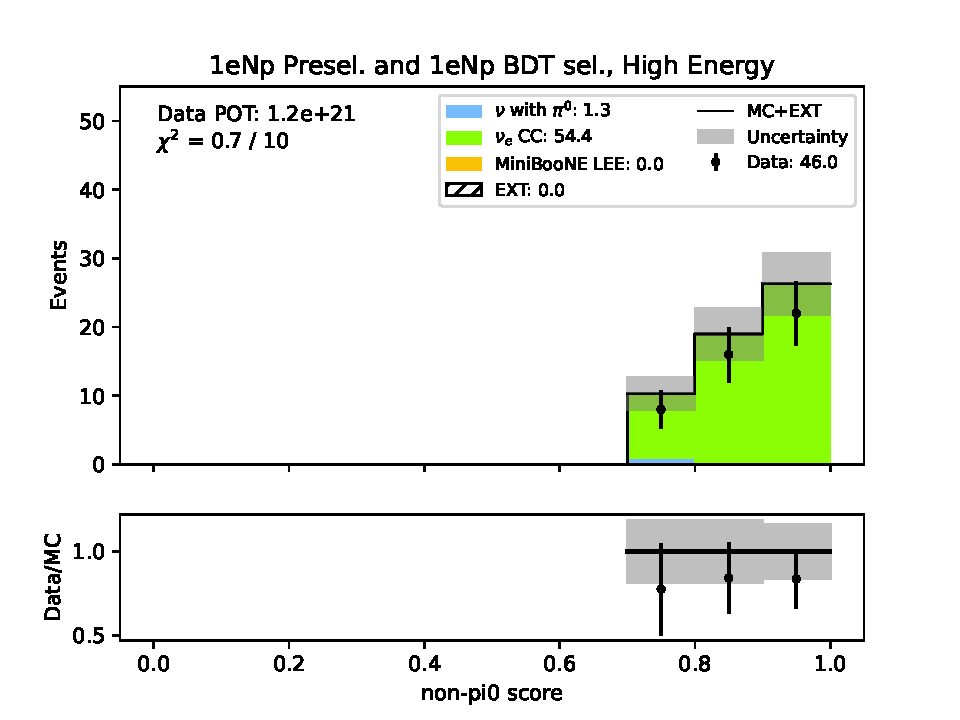
\includegraphics[width=\linewidth]{technote/Sidebands/Figures/FarSideband/far_sideband_nonpi0_score_run1234a4b4c4d5_NP_NPBDT_HIGH_ENERGY.pdf}
    \caption{1eNp BDT selection, runs 1-5.}
    \end{subfigure}
    \caption{Reconstructed neutrino energy in the 1eNp high energy sideband.}
    \label{fig:HighEnergy1eNp_nonpi0_score}
\end{figure}

\begin{figure}[H]
    \centering
    \begin{subfigure}{0.33\linewidth}
    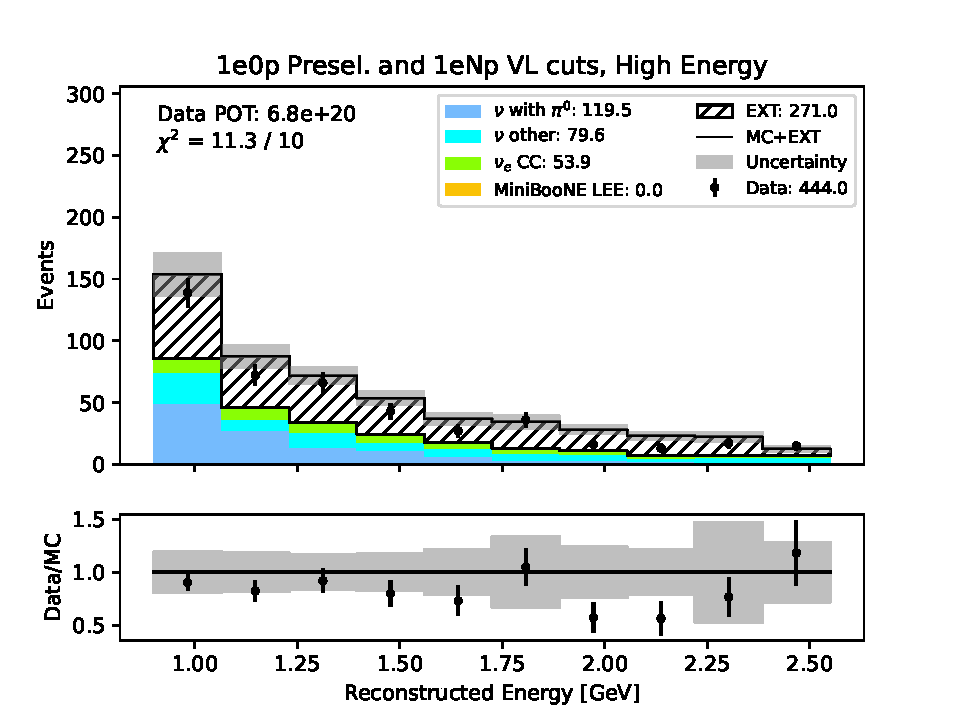
\includegraphics[width=\linewidth]{technote/Sidebands/Figures/FarSideband/far_sideband_reco_e_run123_ZP_ZP_HIGH_ENERGY.pdf}
    \caption{$\nu_e$ preselection, runs 1-3.}
    \end{subfigure}%
    \begin{subfigure}{0.33\linewidth}
    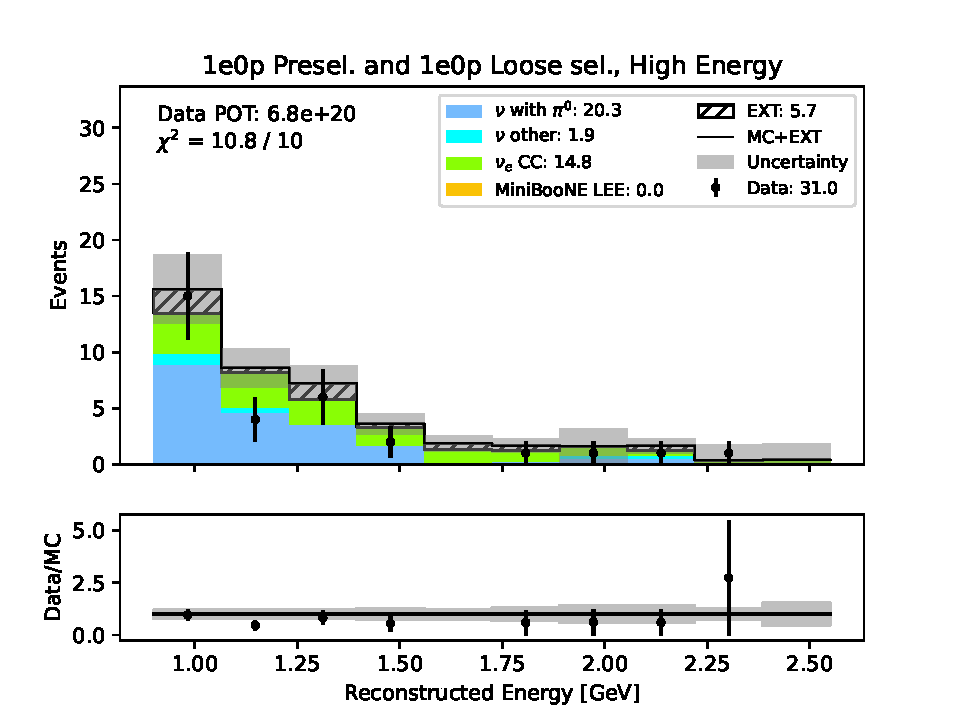
\includegraphics[width=\linewidth]{technote/Sidebands/Figures/FarSideband/far_sideband_reco_e_run123_ZP_ZPLOOSESEL_HIGH_ENERGY.pdf}
    \caption{1e0p loose selection, runs 1-3.}
    \end{subfigure}%
    \begin{subfigure}{0.33\linewidth}
    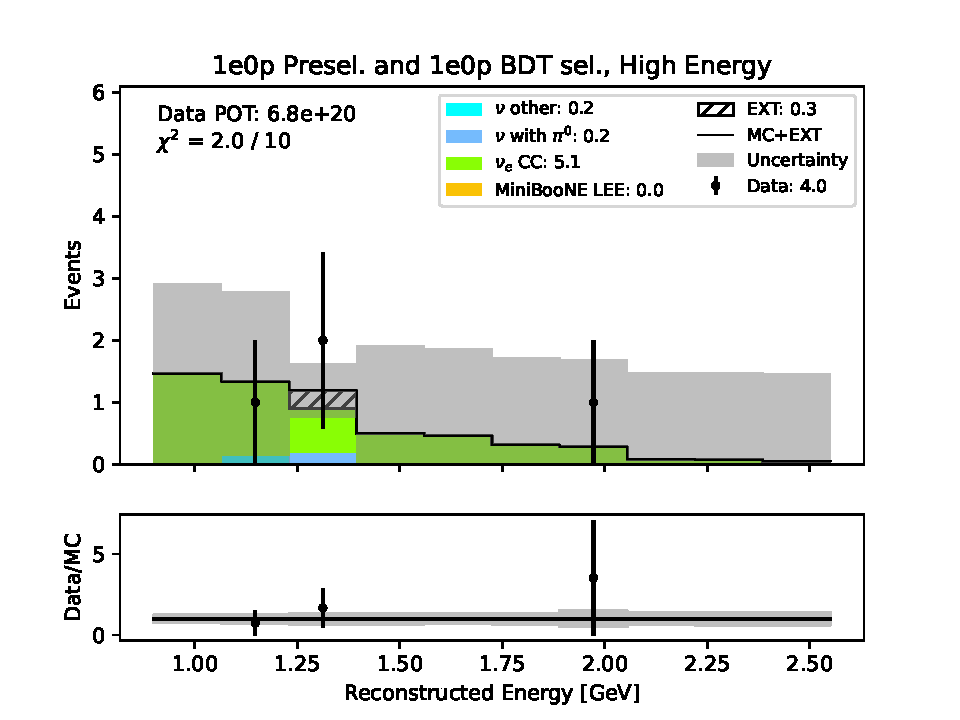
\includegraphics[width=\linewidth]{technote/Sidebands/Figures/FarSideband/far_sideband_reco_e_run123_ZP_ZPBDT_HIGH_ENERGY.pdf}
    \caption{1e0p BDT selection, runs 1-3.}
    \end{subfigure}
    \begin{subfigure}{0.33\linewidth}
    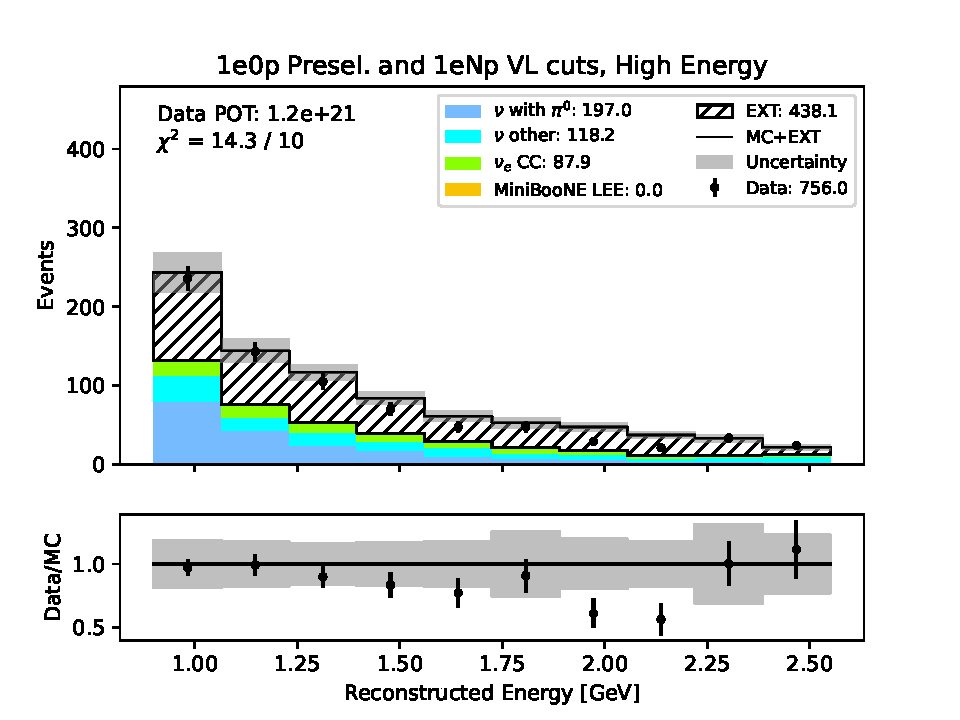
\includegraphics[width=\linewidth]{technote/Sidebands/Figures/FarSideband/far_sideband_reco_e_run1234a4b4c4d5_ZP_ZP_HIGH_ENERGY.pdf}
    \caption{$\nu_e$ preselection., runs 1-5}
    \end{subfigure}%
    \begin{subfigure}{0.33\linewidth}
    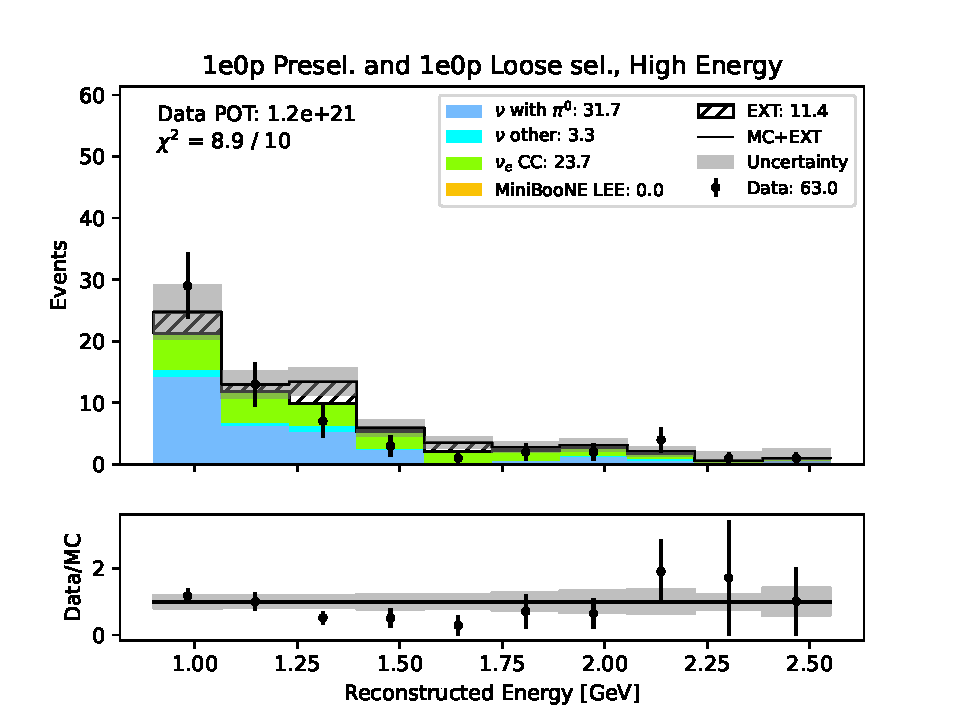
\includegraphics[width=\linewidth]{technote/Sidebands/Figures/FarSideband/far_sideband_reco_e_run1234a4b4c4d5_ZP_ZPLOOSESEL_HIGH_ENERGY.pdf}
    \caption{1e0p loose selection, runs 1-5.}
    \end{subfigure}%
    \begin{subfigure}{0.33\linewidth}
    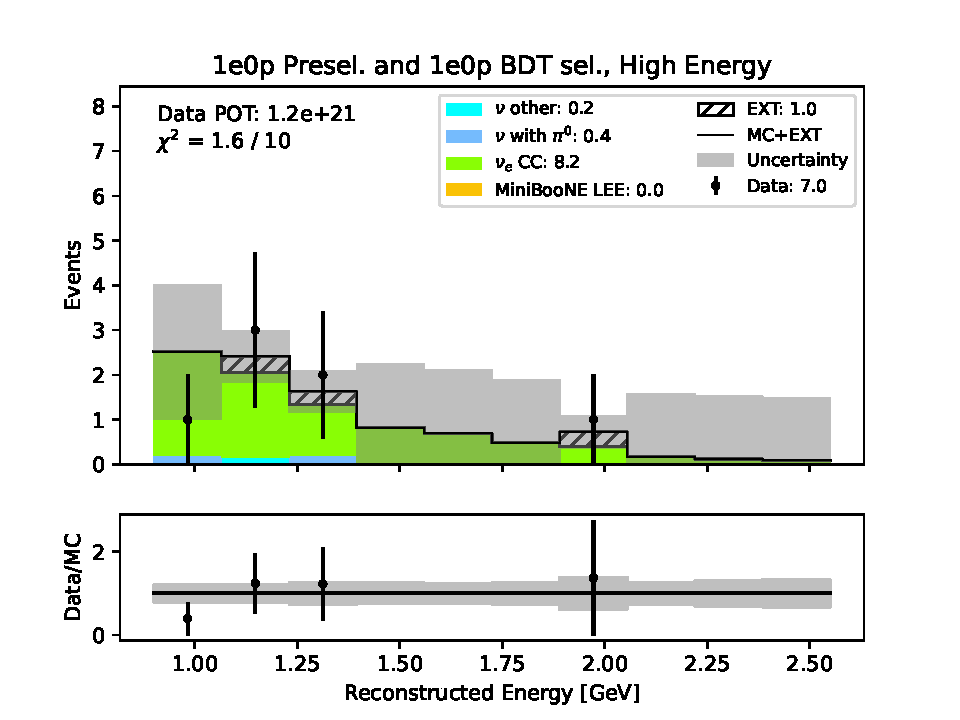
\includegraphics[width=\linewidth]{technote/Sidebands/Figures/FarSideband/far_sideband_reco_e_run1234a4b4c4d5_ZP_ZPBDT_HIGH_ENERGY.pdf}
    \caption{1e0p BDT selection, runs 1-5.}
    \end{subfigure}
    \caption{Reconstructed neutrino energy in the 1e0p high energy sideband.}
    \label{fig:HighEnergy1eNp_nonpi0_score}
\end{figure}

\begin{figure}[H]
    \centering
    \begin{subfigure}{0.33\linewidth}
    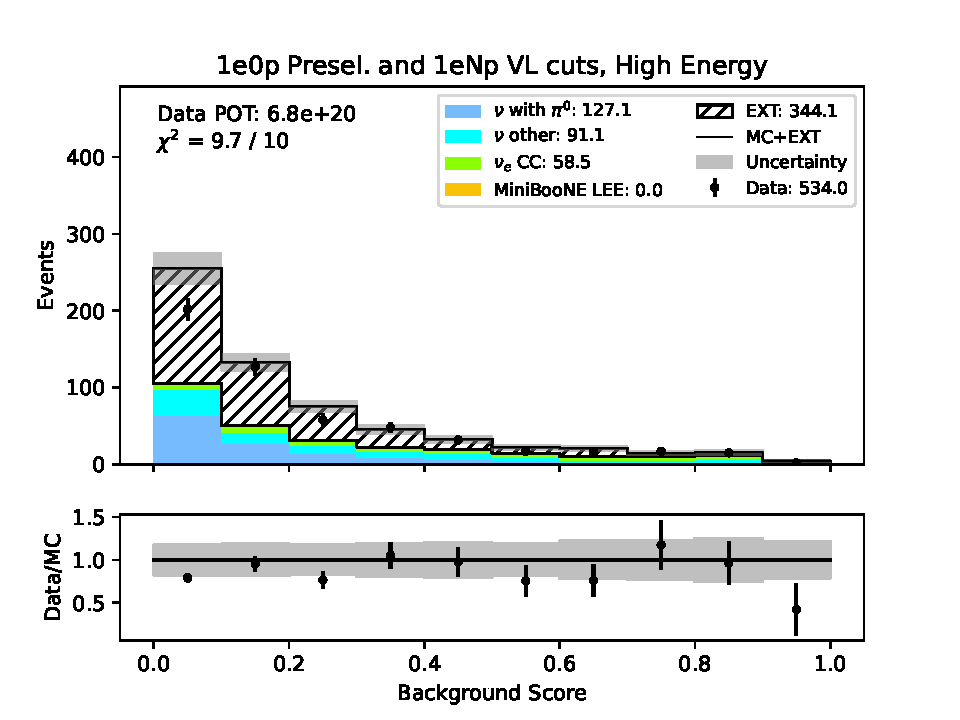
\includegraphics[width=\linewidth]{technote/Sidebands/Figures/FarSideband/far_sideband_bkg_score_run123_ZP_ZP_HIGH_ENERGY.pdf}
    \caption{$\nu_e$ preselection, runs 1-3.}
    \end{subfigure}%
    \begin{subfigure}{0.33\linewidth}
    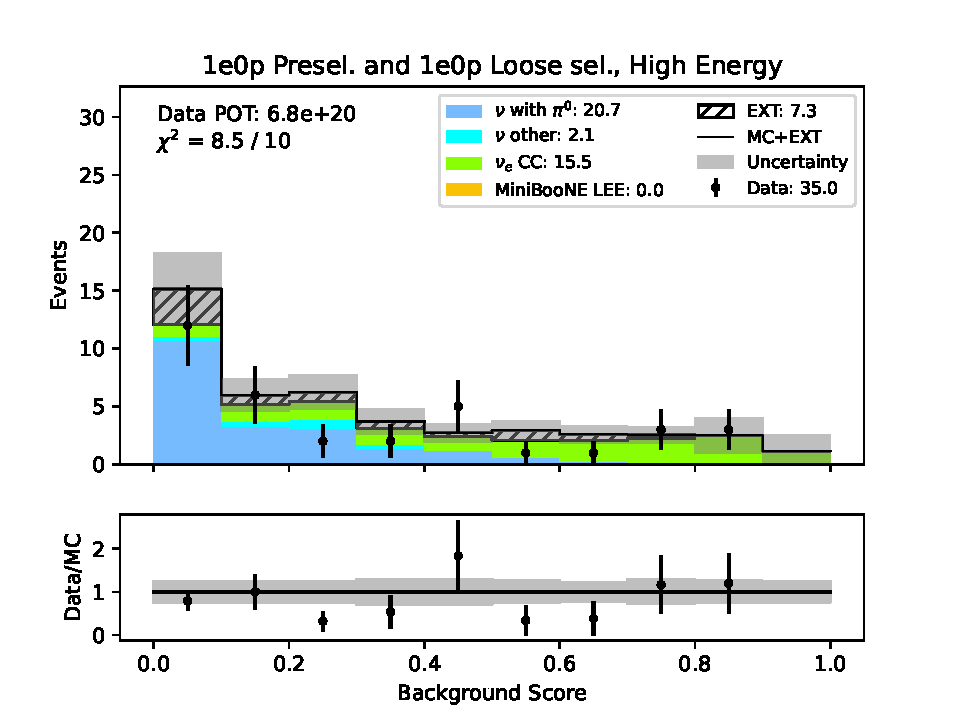
\includegraphics[width=\linewidth]{technote/Sidebands/Figures/FarSideband/far_sideband_bkg_score_run123_ZP_ZPLOOSESEL_HIGH_ENERGY.pdf}
    \caption{1e0p loose selection, runs 1-3.}
    \end{subfigure}%
    \begin{subfigure}{0.33\linewidth}
    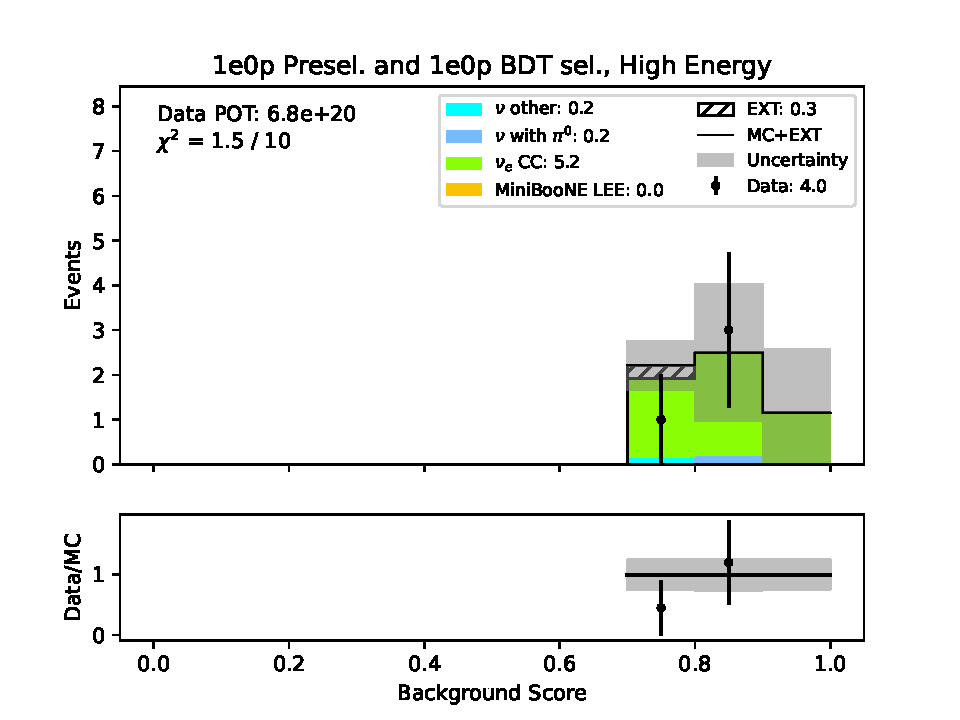
\includegraphics[width=\linewidth]{technote/Sidebands/Figures/FarSideband/far_sideband_bkg_score_run123_ZP_ZPBDT_HIGH_ENERGY.pdf}
    \caption{1e0p BDT selection, runs 1-3.}
    \end{subfigure}
    \begin{subfigure}{0.33\linewidth}
    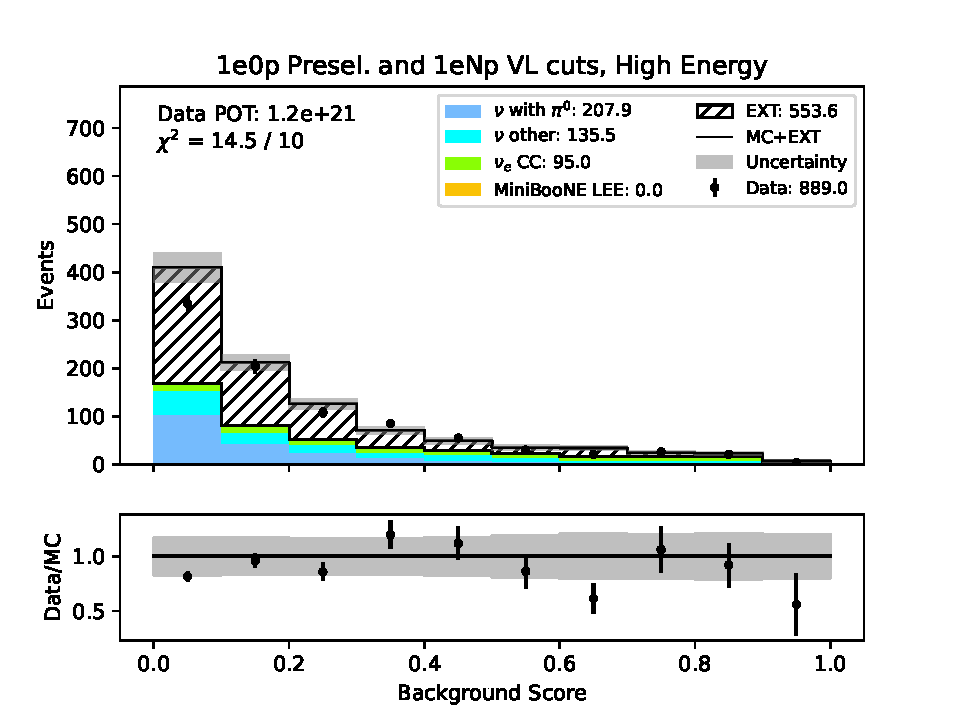
\includegraphics[width=\linewidth]{technote/Sidebands/Figures/FarSideband/far_sideband_bkg_score_run1234a4b4c4d5_ZP_ZP_HIGH_ENERGY.pdf}
    \caption{$\nu_e$ preselection, runs 1-5.}
    \end{subfigure}%
    \begin{subfigure}{0.33\linewidth}
    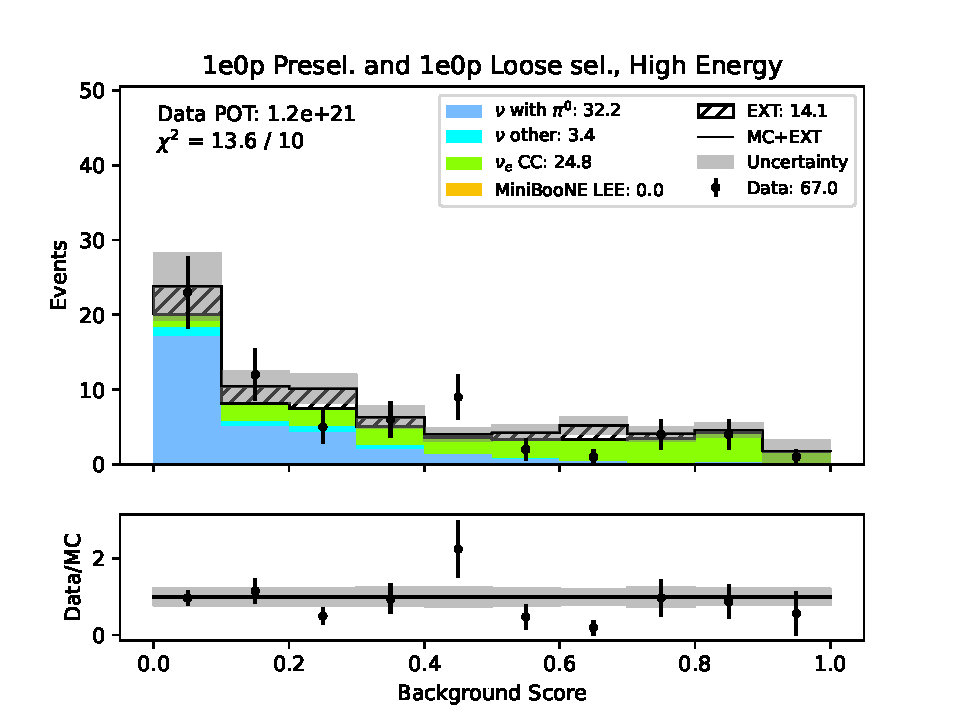
\includegraphics[width=\linewidth]{technote/Sidebands/Figures/FarSideband/far_sideband_bkg_score_run1234a4b4c4d5_ZP_ZPLOOSESEL_HIGH_ENERGY.pdf}
    \caption{1e0p loose selection, runs 1-5.}
    \end{subfigure}%
    \begin{subfigure}{0.33\linewidth}
    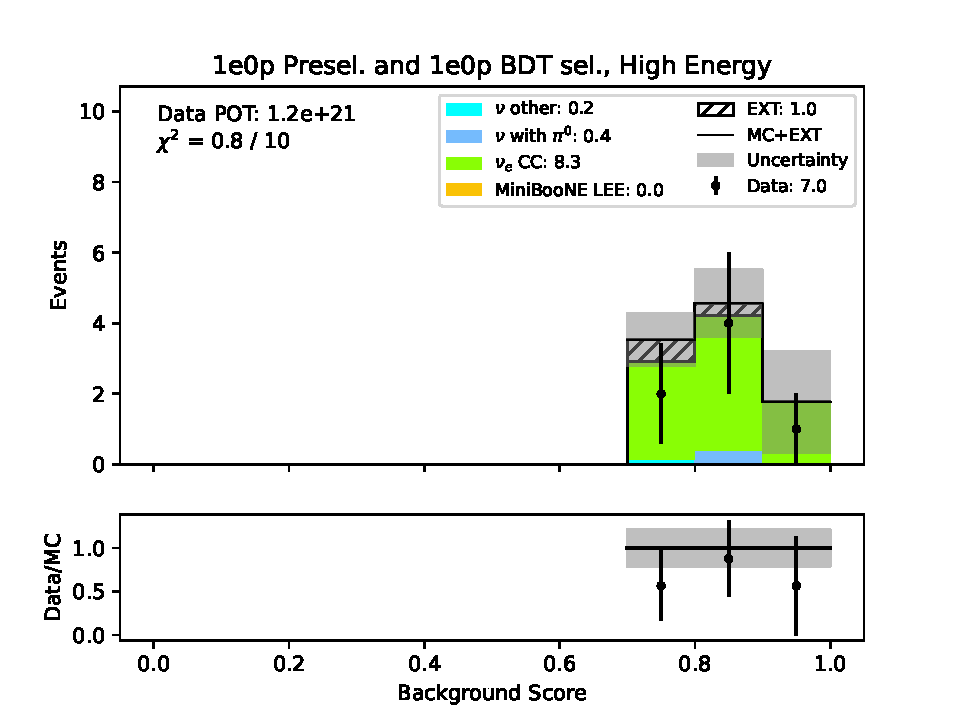
\includegraphics[width=\linewidth]{technote/Sidebands/Figures/FarSideband/far_sideband_bkg_score_run1234a4b4c4d5_ZP_ZPBDT_HIGH_ENERGY.pdf}
    \caption{1e0p BDT selection, runs 1-5.}
    \end{subfigure}
    \caption{Reconstructed neutrino energy in the 1e0p high energy sideband.}
    \label{fig:HighEnergy1eNp_nonpi0_score}
\end{figure}